\begin{frame}{Capital Structure: What Limits the Use of Debt?}
	\small
	\textbf{Beyond Tax Shields — Why Don't Firms Use 100\% Debt?}
	\small
	In this section, we explore factors that challenge the simple tax-based view of optimal capital structure:
	\vspace{-3mm}
	
	\begin{itemize}
		\item \textbf{Case III: Trade-Off Theory}  
		Firms weigh the tax benefits of debt against the costs of financial distress.
		
		\item \textbf{Signaling Effects}  
		Capital structure choices can signal private information to investors.
		\item \textbf{Agency Costs of Equity}  
		Equity financing may create incentive misalignments between owners and managers.
		
		\item \textbf{Pecking Order Theory}  
		Firms prefer internal funds, then debt, and issue equity only as a last resort.
		
		\item \textbf{Real-World Constraints}  
		Legal, institutional, and industry-specific frictions matter too.
	\end{itemize}
	\vspace{-3mm}
	\begin{alertblock}{Goal of This Section}
		To understand why real-world firms often choose \textbf{moderate} debt levels — not extremes.
	\end{alertblock}
	
\end{frame}

\subsection{Costs of Financial Distress}
\begin{frame}{The Downside of Debt: Financial Distress}
	
	\begin{itemize}
		\item Debt creates tax benefits — but also introduces fixed obligations.
		\item \textbf{Failure to meet interest or principal payments leads to distress.}
		\item Ultimate form of distress: \textbf{Bankruptcy}
		\begin{itemize}
			\item Control of assets transfers from shareholders to creditors.
		\end{itemize}
		\item In the real world, \textbf{costs of distress may offset the benefits of debt}.
	\end{itemize}
	
	\vspace{0.2cm}
	\begin{alertblock}{Core Idea}
		There is a trade-off between tax shields and financial distress costs.
	\end{alertblock}
	
\end{frame}

\begin{frame}{Illustration: Bankruptcy Pressure}
	
	\textbf{Cash Flow Uncertainty:}
	
	\begin{itemize}
		\item EBIT = \$100 (Boom) or \$50 (Recession), each with 50\% probability.
		\item Knight Corp: debt requires \$49 in payments.
		\item Day Corp: debt requires \$60 in payments.
	\end{itemize}
	
	\vspace{0.2cm}
	\begin{table}
		\centering
		\caption*{\textbf{Cash Flow Distribution (No Legal Fees)}}
		\begin{tabular}{@{}lcccc@{}}
			\toprule
			& \multicolumn{2}{c}{\textit{Knight Corp}} & \multicolumn{2}{c}{\textit{Day Corp}} \\
			& Boom & Recession & Boom & Recession \\ \midrule
			Firm Cash Flow & \$100 & \$50 & \$100 & \$50 \\
			To Bondholders & \$49 & \$49 & \$60 & \$50 \\
			To Shareholders & \$51 & \$1 & \$40 & \$0 \\ \bottomrule
		\end{tabular}
	\end{table}
	
	\vspace{0.2cm}
	\textbf{Observation:}  
	Day Corp’s higher leverage reduces shareholder value and increases distress risk.
\end{frame}

\begin{frame}{Realistic Scenario: Legal Costs of Distress}
	
	\textbf{In Distress, Lawyers Get Paid First}
	
	\begin{itemize}
		\item Legal battles reduce available cash flow — even before creditors are paid.
		\item Suppose bankruptcy/legal fees = \$15 in recession scenario.
	\end{itemize}
	
	\vspace{0.2cm}
	\begin{table}
		\centering
		\caption*{\textbf{Day Corp with Legal Costs}}
		\begin{tabular}{@{}lcc@{}}
			\toprule
			& Boom & Recession \\ \midrule
			Cash Flow & \$100 & \$50 \\
			To Bondholders & \$60 & \$35 \\
			To Shareholders & \$40 & \$0 \\ \bottomrule
		\end{tabular}
	\end{table}
	
	\vspace{0.2cm}
	\textbf{Conclusion:}  
	Distress reduces total value available to claimholders — debt becomes costly.
\end{frame}

\begin{frame}{Direct Costs of Financial Distress}
	
	\textbf{Legal and Administrative Costs:}
	\begin{itemize}
		\item Legal fees during reorganization or liquidation can be substantial.
		\item Enron: \$1 billion; WorldCom: \$600 million
		\item These costs are paid before creditors or shareholders receive anything.
	\end{itemize}
	
	\vspace{0.3cm}
	\textbf{Empirical Estimates:}
	\begin{itemize}
		\item \textcite{white1980bankruptcy}: Direct costs $\approx$ 3\% of firm value
		\item \textcite{warner1977bankruptcy}: Average $\approx$ 1\% of firm value (7 years before bankruptcy)
	\end{itemize}
	
	\vspace{0.3cm}
	\begin{alertblock}{Key Point}
		Even small percentage costs can erode tax benefits when distress probability is high.
	\end{alertblock}
	
\end{frame}

\begin{frame}{Indirect Costs of Financial Distress}
	
	\textbf{Harder to Observe — Still Very Real:}
	\begin{itemize}
		\item Loss of customers or suppliers
		\item Difficulty attracting or retaining talent
		\item Strategic delays or loss of growth opportunities
	\end{itemize}
	
	\vspace{0.3cm}
	\textbf{Example: GM \& Chrysler (2008)}
	\begin{itemize}
		\item 75\% of surveyed consumers said they wouldn’t buy from a bankrupt carmaker.
		\item Financial distress amplified by loss of confidence.
	\end{itemize}
	
	\vspace{0.3cm}
	\textbf{Key Feature:}  
	Difficult to measure — but can far exceed direct costs.
	
\end{frame}

\subsubsection{Agency Costs: Equity vs. Debt Conflict}
\begin{frame}{Agency Costs: Equity vs. Debt Conflict}
	
	\textbf{When a firm issues debt, the interests of stockholders and bondholders diverge.}
	
	\begin{itemize}
		\item Equityholders may pursue \textbf{self-serving strategies} that shift value from creditors.
		\item These strategies increase the risk of default, reduce firm value, and are especially problematic near distress.
		\item The resulting value loss is known as an \textbf{agency cost of debt}.
	\end{itemize}
	
	\vspace{0.3cm}
	\begin{block}{Three Common Selfish Strategies}
		\begin{enumerate}
			\item Excessive risk-taking (gamble for resurrection)
			\item Underinvestment (debt overhang)
			\item Asset stripping or “milking the property”
		\end{enumerate}
	\end{block}
	
\end{frame}

\begin{frame}{Case: Company in Financial Distress}
	
	\textbf{Balance Sheet of a Distressed Firm}
	
	\begin{table}
		\centering
		\begin{tabular}{@{}llllll@{}}
			\toprule
			Assets      & BV    & MV    & Liabilities & BV    & MV    \\ \midrule
			Cash        & \$200 & \$200 & Bonds       & \$300 & \$200 \\
			Fixed Assets & \$400 & \$0   & Equity      & \$300 & \$0   \\
			Total       & \$600 & \$200 & Total       & \$600 & \$200 \\ \bottomrule
		\end{tabular}
	\end{table}
	
	\begin{itemize}
		\item Liquidation today: Bondholders receive all \$200 → Shareholders get \textbf{nothing}.
		\item But shareholders control investment decisions.
	\end{itemize}
	
\end{frame}

\begin{frame}{Selfish Strategy 1: Excessive Risk-Taking}
	
	\textbf{The Gamble: Use all \$200 cash for a risky investment}
	
	\begin{table}
		\centering
		\begin{tabular}{lll}
			\toprule
			Outcome     & Probability & Payoff \\ \midrule
			Win Big     & 10\%        & \$1,000 \\
			Lose All    & 90\%        & \$0 \\ \bottomrule
		\end{tabular}
	\end{table}
	
	\vspace{0.2cm}
	\begin{itemize}
		\item Required return = 50\%, investment cost = \$200
		\item Expected payoff = \$100 → NPV = \(-133\)
	\end{itemize}
	
	\vspace{0.2cm}
	\begin{equation*}
		\text{NPV} = -200 + \frac{100}{1.5} = -133
	\end{equation*}
	
	\begin{alertblock}{Insight}
		The firm destroys value, but equityholders benefit in the up-state.
	\end{alertblock}
	
\end{frame}

\begin{frame}{Value Shift from Bondholders to Stockholders}
	
	\begin{itemize}
		\item \textbf{Expected CF Distribution}:
		\begin{itemize}
			\item To Bondholders: \$30 → PV = \$20
			\item To Stockholders: \$70 → PV = \$47
		\end{itemize}
		
		\item \textbf{Compare to status quo:}
		\begin{itemize}
			\item PV of Bonds (no gamble) = \$200
			\item PV of Stock = \$0
		\end{itemize}
	\end{itemize}
	
	\begin{alertblock}{Conclusion}
		Equityholders shift value from bondholders → destroy firm value.
	\end{alertblock}
	
\end{frame}


\begin{frame}{Selfish Strategy 2: Underinvestment (Debt Overhang)}
	
	\begin{block}{The Problem}
		Equityholders refuse to invest in value-enhancing projects that mostly benefit bondholders.
	\end{block}
	
	\begin{itemize}
		\item Project: Cost = \$300 → PV = \$318.18
		\item Required capital = \$100 from shareholders
		\item Return to firm > cost, but return to shareholders is negative
	\end{itemize}
	
	\begin{equation*}
		\text{NPV} = -300 + \frac{350}{1.1} = 18.18 > 0
	\end{equation*}
	
\end{frame}

\begin{frame}{Underinvestment: Who Gets What?}
	
	\begin{itemize}
		\item \textbf{Payoffs:}
		\begin{itemize}
			\item Bondholders: \$300 → PV = \$272.73
			\item Shareholders: \$50 → PV = \$45.45
			\item But \$100 out-of-pocket → Net PV to shareholders = \textbf{-\$54.55}
		\end{itemize}
		
		\item \textbf{Result:} Shareholders rationally reject positive-NPV project.
		
	\end{itemize}
	
	\begin{alertblock}{Outcome}
		Project creates value for the firm — but not for shareholders.
	\end{alertblock}
	
\end{frame}

\begin{frame}{Selfish Strategy 3: Milking the Property}
	
	\textbf{Tactics to extract value before bankruptcy:}
	
	\begin{itemize}
		\item \textbf{Liquidating dividends:}
		\begin{itemize}
			\item Firm pays out \$200 dividend to shareholders
			\item Leaves bondholders with no recovery value
			\item Often violates bond covenants
		\end{itemize}
		
		\item \textbf{Excessive perquisites:}
		\begin{itemize}
			\item Use corporate resources for personal consumption
			\item Hard to monitor, especially in privately held firms
		\end{itemize}
	\end{itemize}
	
	\begin{alertblock}{Key Issue}
		Shareholders extract private benefits — even if firm enters default.
	\end{alertblock}
	
\end{frame}

\begin{frame}{Summary: Who Pays for Selfish Behavior?}
	
	\begin{itemize}
		\item These distortions arise primarily when:
		\begin{itemize}
			\item Firm is highly leveraged
			\item Distress or default is likely
		\end{itemize}
		
		\item \textbf{Bondholders react:}
		\begin{itemize}
			\item Raise required yield
			\item Demand covenants
		\end{itemize}
		
		\item \textbf{Stockholders ultimately pay:}
		\begin{itemize}
			\item Higher cost of debt reduces equity value
			\item Financing becomes expensive or inaccessible
		\end{itemize}
	\end{itemize}
	
	\vspace{0.3cm}
	\begin{alertblock}{Conclusion}
		Agency conflicts raise the effective cost of debt — and limit a firm’s ability to borrow.
	\end{alertblock}
	
\end{frame}

\subsubsection{Mitigating Agency Conflicts Between Shareholders and Creditors}
\begin{frame}{Mitigating Conflict: Protective Covenants}
	
	\textbf{Bond Covenants} are contractual restrictions designed to align stockholder and bondholder interests by reducing agency costs.
	
	\begin{block}{Types of Covenants}
		\begin{itemize}
			\item \textbf{Negative Covenants:} Prohibit risky actions
			\begin{itemize}
				\item No sale or lease of major assets without approval
				\item No issuance of additional long-term debt
			\end{itemize}
			
			\item \textbf{Positive Covenants:} Require prudent behavior
			\begin{itemize}
				\item Maintain minimum levels of working capital
				\item Provide regular financial statements
			\end{itemize}
		\end{itemize}
	\end{block}
	
	\vspace{0.2cm}
	\textbf{Tradeoff:}  
	Though they reduce financial flexibility, covenants can lower borrowing costs and increase firm value by protecting creditor claims.
	
\end{frame}
\begin{frame}{Mitigating Conflict: Debt Coordination and Hybrid Claims}
	
	\textbf{Debt Consolidation Reduces Conflict Among Creditors}
	
	\begin{itemize}
		\item Bankruptcy costs rise when multiple creditors compete for limited assets.
		\item Solution: Fewer, centralized creditors → Easier negotiation in distress.
		\item Example: One lead lender finances all long-term debt.
	\end{itemize}
	
	\vspace{0.3cm}
	\textbf{Blending Stakeholder Roles}
	
	\begin{itemize}
		\item Encourage \textbf{creditor equity ownership}: debt holders also hold shares
		\item Aligns incentives — both care about total firm value, not just claim-specific returns
		\item Common in restructurings, PE-backed LBOs, or convertible bond structures
	\end{itemize}
	
	\vspace{0.2cm}
	\begin{alertblock}{Goal}
		Reduce value-destroying conflicts by integrating or coordinating stakeholder interests.
	\end{alertblock}
	
\end{frame}

\begin{frame}{Looking Ahead: Broader Mechanism Design}
	
	While protective covenants and creditor coordination help reduce agency conflicts, modern corporate finance also utilizes other contractual tools:
	
	\begin{itemize}
		\item \textbf{Convertible Bonds}: align incentives by letting creditors participate in upside.
		\item \textbf{Performance-Based Covenants}: dynamically adjust restrictions based on financial ratios.
		\item \textbf{Equity Issuance}: may serve as a signal of management confidence — or distress.
	\end{itemize}
	
	\vspace{0.3cm}
	\begin{alertblock}{Next}
		These institutional designs help mitigate the costs of debt, but they do not eliminate them.  
		We now turn to the broader \textbf{Trade-Off Theory}, which balances benefits (like tax shields) with costs (like financial distress and agency).
	\end{alertblock}
	
\end{frame}

\subsection{Trade-Off Theory of Capital Structure}
\begin{frame}{The Static Trade-Off Theory}
	
	\begin{itemize}
		\item Firms trade off the benefits of debt (tax shields) against the costs of financial distress.
		\item \textbf{Static Trade-Off Theory:}  
		Borrowing continues until:
		\[
		\text{Marginal Tax Shield} = \text{Marginal Distress Cost}
		\]
	\end{itemize}
	\vspace{-3mm}
	\begin{figure}
		\centering
		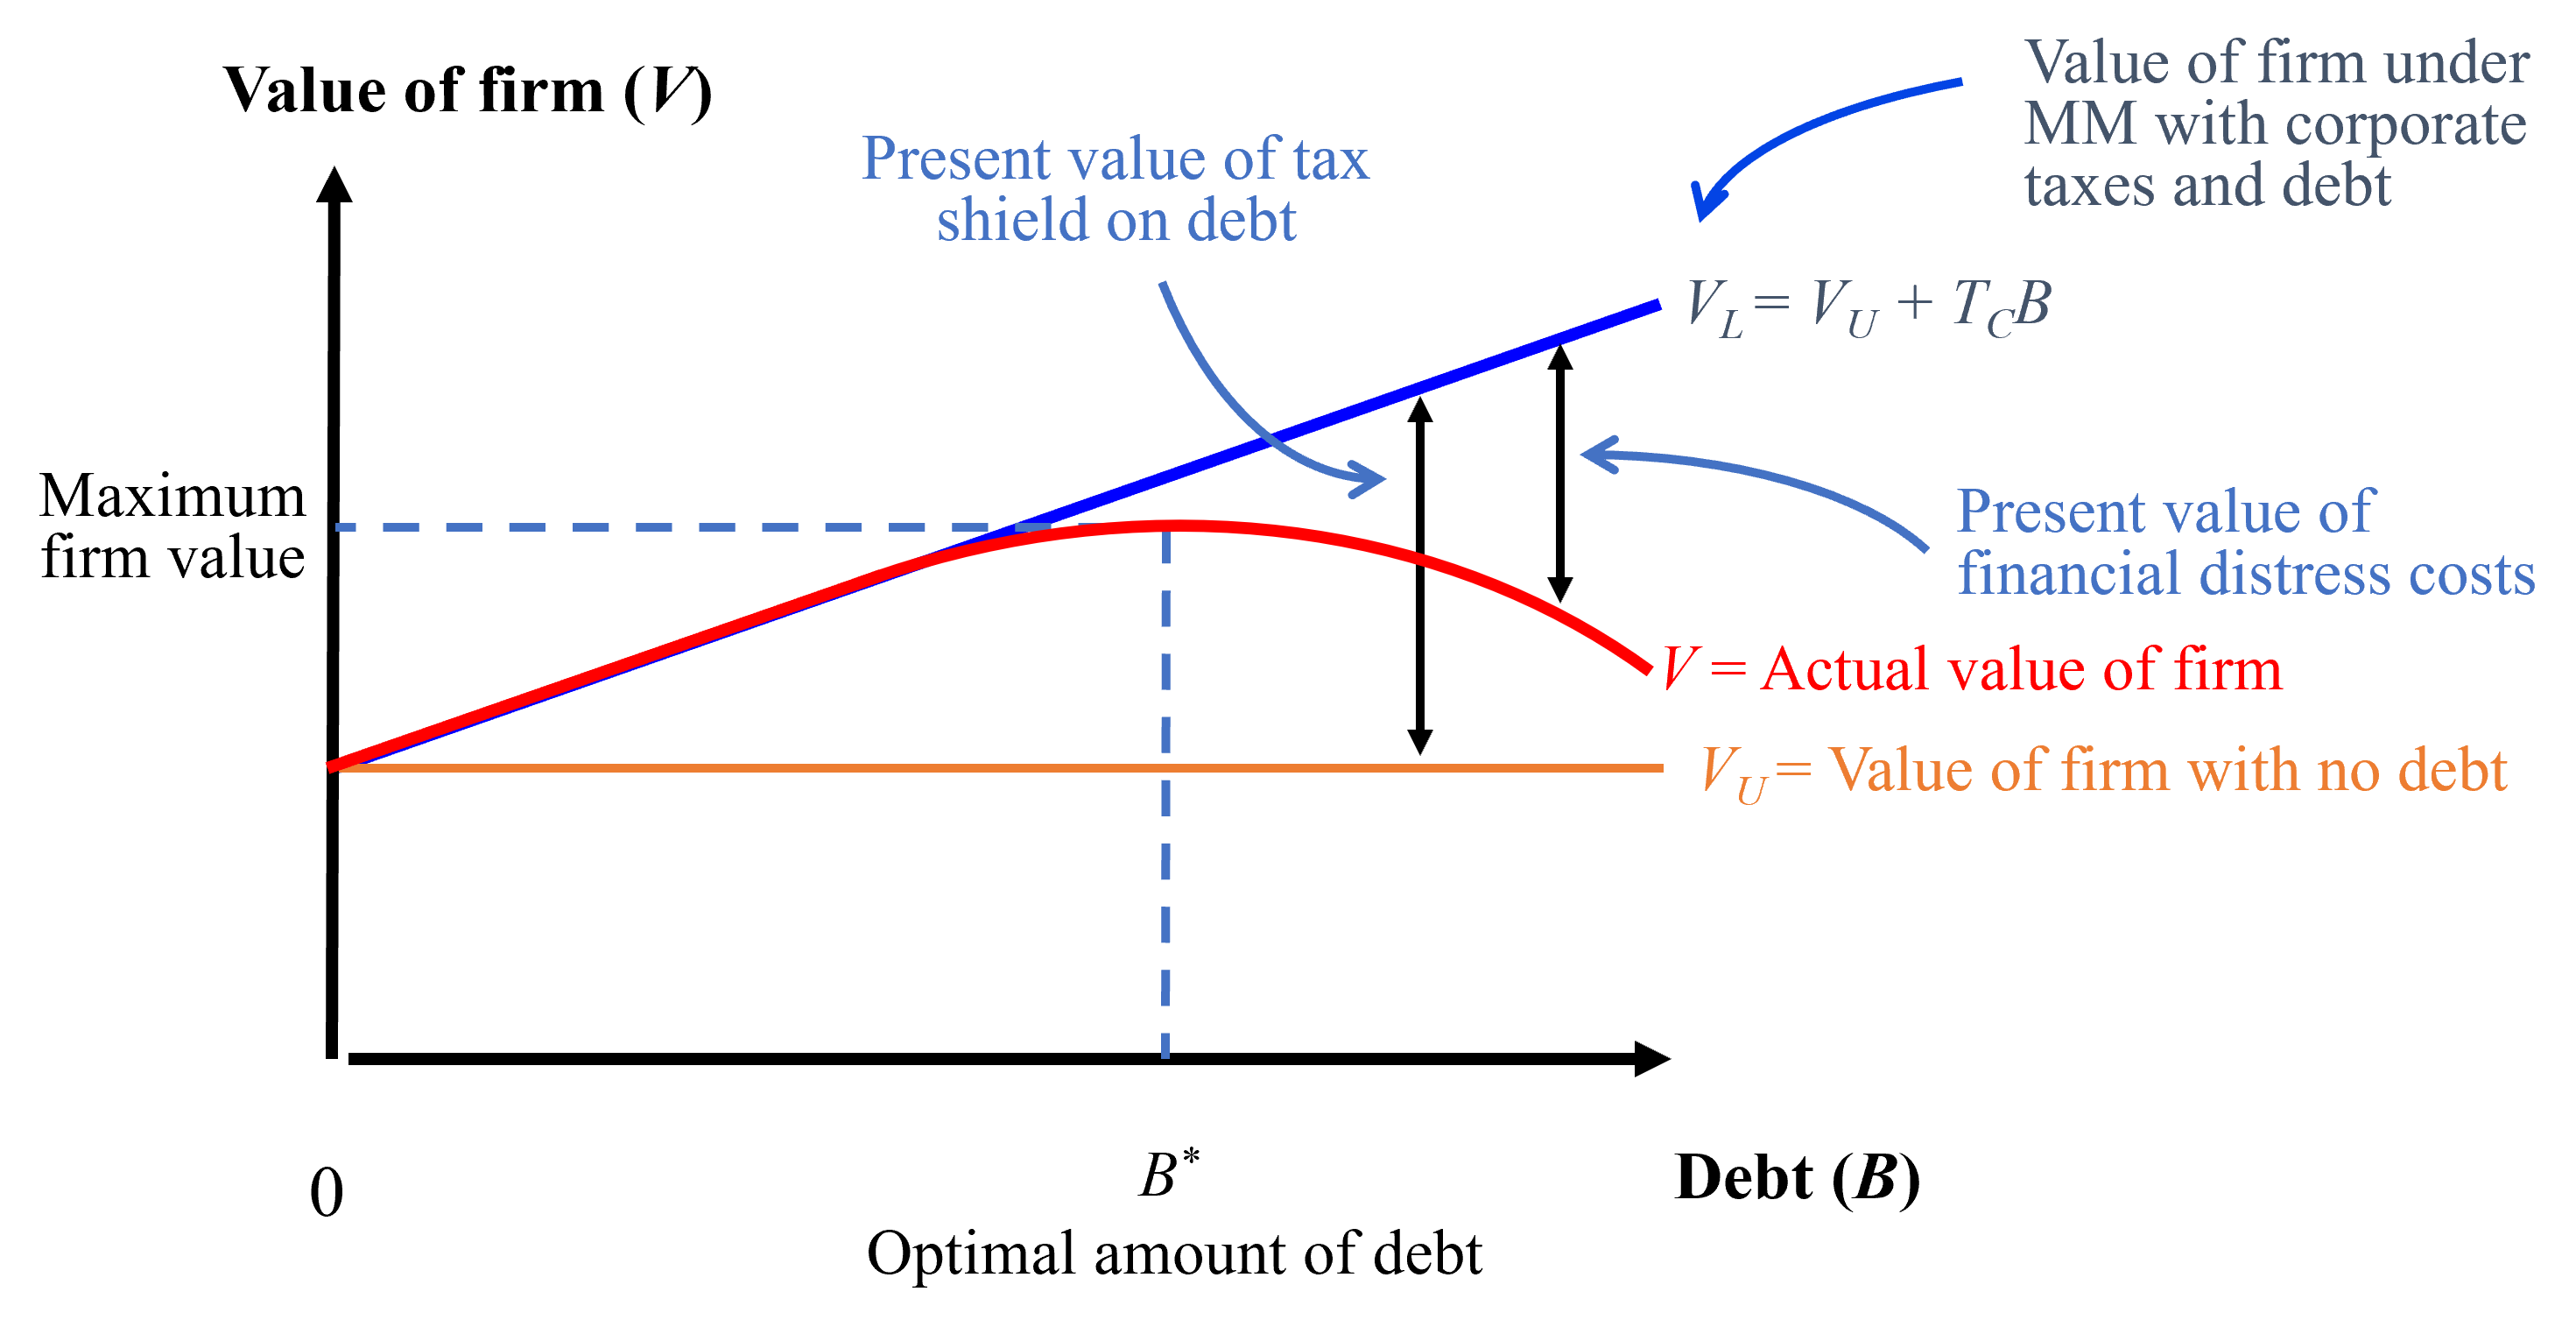
\includegraphics[width=0.7\textwidth]{images/section3/optimaldbratio.png}
		\caption*{\tiny Optimal capital structure occurs before distress costs outweigh tax benefits}
	\end{figure}
	
\end{frame}

\begin{frame}{WACC and the Optimal Capital Structure}
	
	\begin{columns}
		\column{0.52\textwidth}
		\begin{itemize}
			\item The capital structure that \textbf{maximizes firm value} is also the one that \textbf{minimizes WACC}.
			\item Initially, debt lowers WACC due to:
			\begin{itemize}
				\item Lower after-tax cost of debt
			\end{itemize}
			\item Beyond a certain point:
			\begin{itemize}
				\item Higher debt → higher risk → higher \( R_D \) and \( R_E \)
				\item WACC starts to rise
			\end{itemize}
		\end{itemize}
		
		\column{0.48\textwidth}
		\begin{figure}
			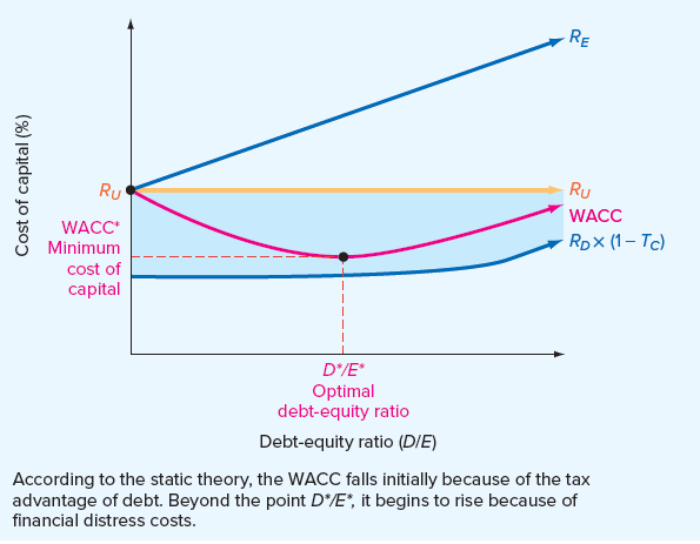
\includegraphics[width=\linewidth]{images/section3/minimalwacc.png}
		\end{figure}
		
	\end{columns}
	
\end{frame}

\begin{frame}{Summary: M\&M Cases and Optimal Capital Structure}
	
	\begin{itemize}
		\item \textbf{Case I: No Taxes, No Bankruptcy Costs}
		\begin{itemize}
			\item Firm value independent of capital structure
			\item \textcolor{gray}{→ No optimal capital structure}
		\end{itemize}
		
		\vspace{2mm}
		\item \textbf{Case II: Corporate Taxes Only}
		\begin{itemize}
			\item Debt creates tax shields → increases firm value
			\item \textcolor{gray}{→ Optimal capital structure = nearly 100\% debt}
		\end{itemize}
		
		\vspace{2mm}
		\item \textbf{Case III: Taxes + Distress Costs}
		\begin{itemize}
			\item Value of debt is offset by expected cost of distress
			\item \textcolor{gray}{→ Optimal capital structure: part debt, part equity}
		\end{itemize}
	\end{itemize}
	
	\vspace{0.2cm}
	\begin{alertblock}{Bottom Line}
		Capital structure matters only when frictions like taxes and bankruptcy costs are present.
	\end{alertblock}
	
\end{frame}

\begin{frame}{M\&M Framework: Comparing Case I, II, and III}
	
	\begin{table}[ht]
		\centering
		\resizebox{\textwidth}{!}{
			\begin{tabular}{lccc}
				\toprule
				\textbf{Dimension} & \textbf{Case I} & \textbf{Case II} & \textbf{Case III} \\
				\midrule
				Taxes & \faTimesCircle None & \faCheckCircle Corporate taxes & \faCheckCircle Corporate taxes \\
				Bankruptcy Costs & \faTimesCircle None & \faTimesCircle None & \faCheckCircle Present \\
				\midrule
				Effect of Debt on Firm Value & None & Increases value via tax shield & Increases value, but with diminishing returns \\
				Optimal Capital Structure & Irrelevant & Almost 100\% debt & Moderate debt level \\
				Cost of Equity \(R_S\) & Increases with leverage & Increases with leverage & Increases faster due to distress risk \\
				WACC & Constant & Decreases with debt & U-shaped: minimized at intermediate debt \\
				\bottomrule
			\end{tabular}
		}
	\end{table}
	
	\vspace{0.2cm}
	\begin{alertblock}{Key Insight}
		Debt is most valuable in Case II. In the real world (Case III), the optimal capital structure is a trade-off between tax benefits and distress costs.
	\end{alertblock}
	
\end{frame}


\begin{frame}{Managerial Implications for Capital Structure}
	
	\textbf{How should managers think about debt?}
	
	\begin{itemize}
		\item \textbf{Tax Position of the Firm}
		\begin{itemize}
			\item Firms with higher and stable taxable income benefit more from debt.
		\end{itemize}
		
		\item \textbf{Financial Distress Risk}
		\begin{itemize}
			\item Firms with volatile EBIT or low asset tangibility should use less debt.
			\item Industry-specific distress costs can vary significantly.
		\end{itemize}
		
		\item \textbf{Practical Guidance:}
		\begin{itemize}
			\item No “one-size-fits-all” solution.
			\item Capital structure must reflect firm fundamentals and risk tolerance.
		\end{itemize}
	\end{itemize}
	
\end{frame}

\subsection{The Extended Pie Model and Broader Stakeholder Claims}
\begin{frame}{The Extended Pie Model: Cash Flows and All Stakeholders}
	
	\textbf{Core Idea:}  
	Capital structure decisions affect not just shareholders and bondholders, but all claimants on the firm’s cash flows.
	
	\vspace{0.3cm}
	\begin{itemize}
		\item \textbf{Taxes:}  
		Increased debt reduces taxes — decreasing the government’s claim on cash flows.
		
		\item \textbf{Bankruptcy Costs:}  
		As leverage increases, the expected value of legal and administrative costs rises.
		
		\item \textbf{All Claims Come from One Source:}
		\[
		\begin{aligned}
			CF &= \text{SUM(stockholders + creditors + gov + courts + others)}
		\end{aligned}
		\]
	\end{itemize}
	
	\vspace{0.3cm}
	\begin{alertblock}{Extended Pie View}
		The firm’s total cash flow supports both \textit{marketed} and \textit{nonmarketed} claims.
	\end{alertblock}
	
\end{frame}

\begin{frame}{The Extended Pie: A Visual Perspective}
	
	\begin{figure}
		\centering
		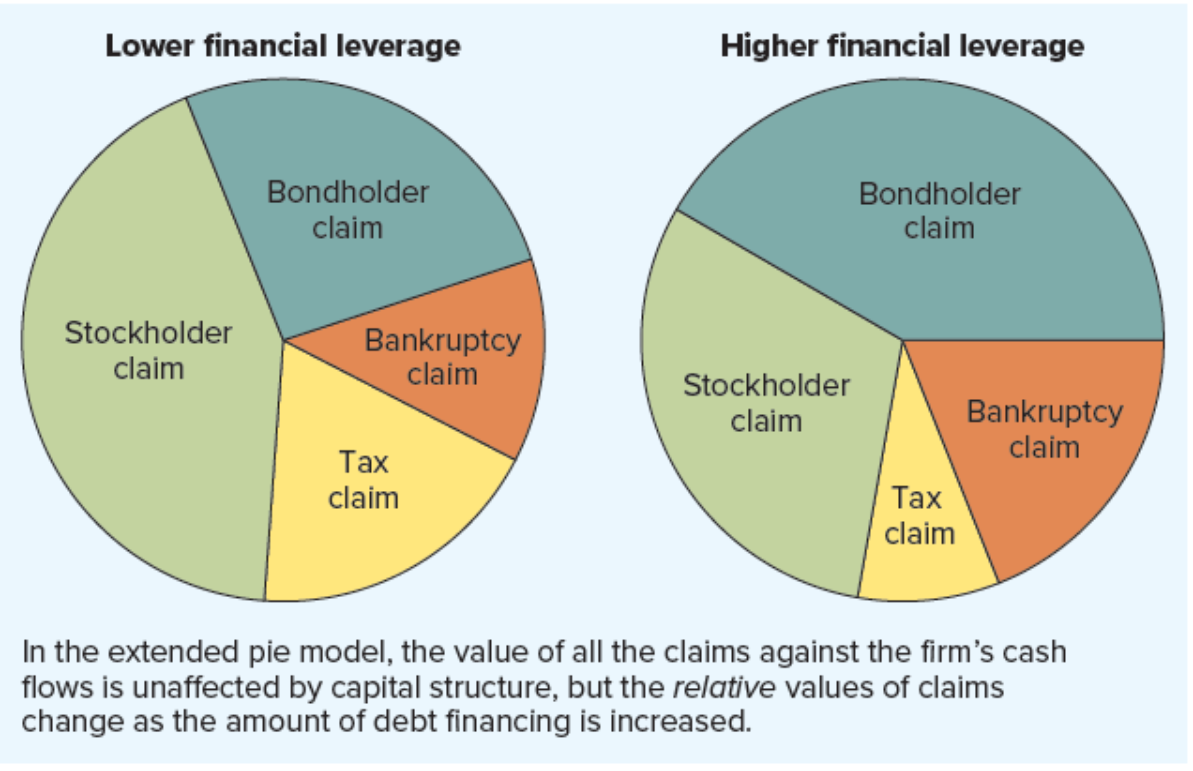
\includegraphics[width=0.9\textwidth]{images/section3/pieII}
	\end{figure}
	
%	\vspace{0.3cm}
%	\textbf{Interpretation:}  
%	When the pie is sliced differently via capital structure changes, the size of some slices (like taxes or distress costs) changes too — affecting marketed claimants.
	
\end{frame}

\begin{frame}{Marketed vs. Nonmarketed Claims}
	
	\textbf{Who has a claim on the firm's cash flows?}
	
	\vspace{0.2cm}
	\begin{itemize}
		\item \textbf{Marketed Claims:}
		\begin{itemize}
			\item Shareholders, bondholders
			\item Traded in financial markets → priced explicitly
		\end{itemize}
		
		\item \textbf{Nonmarketed Claims:}
		\begin{itemize}
			\item Government (taxes), lawyers (bankruptcy fees), communities (externalities)
			\item Cannot be traded but still consume firm resources
		\end{itemize}
	\end{itemize}
	
	\vspace{0.3cm}
	\[
	V_T = V_M + V_N = \text{Total Firm Value}
	\]
	
	\vspace{0.2cm}
	\textbf{Capital structure decisions may shift value between} $V_M$ and $V_N$.
\end{frame}

\begin{frame}{Capital Structure and Broader Stakeholders: A CSR Link}
	
	\textbf{Why Extended Pie Theory Matters in Modern Finance:}
	
	\begin{itemize}
		\item Firms increasingly face scrutiny not just from investors, but also:
		\begin{itemize}
			\item Governments (tax strategies)
			\item Local communities (employment, environmental impacts)
			\item Employees and supply chains
		\end{itemize}
		
		\item \textbf{Capital structure affects these stakeholders:}
		\begin{itemize}
			\item High debt may reduce tax payments, but increase risk to employees or local economies
			\item Aggressive financial policy may reduce long-term reputational capital
		\end{itemize}
	\end{itemize}
	
	\vspace{0.2cm}
	\begin{alertblock}{Strategic Implication}
		The optimal capital structure must increasingly account for \textbf{nonmarketed claims and CSR concerns}.
	\end{alertblock}
	
\end{frame}

\subsection{Beyond Trade-Off: Other Capital Structure Theories}


\subsubsection{Agency Costs of Equity}
\begin{frame}{Agency Costs of Equity: Incentives and Ownership}
	
	\textbf{\textcite{jensen1976theory}} argue that the separation of ownership and control leads to incentive misalignment.
	
	\vspace{0.3cm}
	\begin{itemize}
		\item When managers own a smaller share of the firm (e.g., after issuing new equity), they:
		\begin{itemize}
			\item Have weaker incentives to maximize firm value
			\item May increase consumption of perks or pursue pet projects
			\item May reduce effort or adopt low-value investments
		\end{itemize}
		
		\item Investors anticipate such behavior:
		\begin{itemize}
			\item → New equity may be undervalued in the market
			\item → Managers may avoid issuing equity even when needed
		\end{itemize}
	\end{itemize}
	
	\vspace{0.2cm}
	\begin{alertblock}{Capital Structure Implication}
		Firms with severe equity agency costs may prefer debt to preserve managerial discipline.
	\end{alertblock}
	
\end{frame}


\begin{frame}{Agency Incentives in Action: Ms. Pagell's Dilemma}
	
	\textbf{Owner-manager chooses between debt and equity to raise \$2M.}
	
	\begin{itemize}
		\item More ownership retained under debt → stronger work incentives.
		\item Less ownership under equity → lower incentive to exert effort.
	\end{itemize}
	
	\vspace{0.3cm}
	\begin{table}
		\centering
		\resizebox{0.95\textwidth}{!}{
			\begin{tabular}{@{}lrrrrrrr@{}}
				\toprule
				& & \multicolumn{3}{c}{\textbf{Debt Issue}} & \multicolumn{3}{c}{\textbf{Stock Issue}} \\ \midrule
				\textbf{Work Hours} & \textbf{CF} & \textbf{Interest} & \textbf{Equity CF} & \textbf{To Pagell} & \textbf{Interest} & \textbf{Equity CF} & \textbf{To Pagell} \\
				6-hour/day  & 300K & 240K & 60K & 60K   & 0 & 300K & 100K \\
				10-hour/day & 400K & 240K & 160K & 160K & 0 & 400K & 133K \\
				\bottomrule
			\end{tabular}
		}
	\end{table}
	
\end{frame}

\begin{frame}{Equity Dilution and Incentive Losses}
	
	\begin{itemize}
		\item As equity increases:
		\begin{itemize}
			\item Ownership becomes dispersed
			\item Managers exert less effort
			\item Free cash flow may be wasted
		\end{itemize}
		
		\item \textbf{Equity valuation drops} in anticipation of these behaviors.
		
		\item \textbf{Debt can improve firm value through:}
		\begin{enumerate}
			\item Tax shield benefit
			\item Reducing equity agency costs
			\item But: Increases expected distress costs
		\end{enumerate}
	\end{itemize}
	
\end{frame}

\subsubsection{Free Cash Flow Hypothesis}
\begin{frame}{Free Cash Flow and the Disciplinary Role of Debt}
	
	\begin{block}{Free Cash Flow Hypothesis \parencite{jensen1986agency}}
		Managers overinvest or consume perks when firms have excess free cash flow.
	\end{block}
	
	\vspace{0.3cm}
	\begin{itemize}
		\item \textbf{Higher Dividends}: Reduces cash under managerial control.
		\item \textbf{Higher Debt}:  
		\begin{itemize}
			\item Forces regular payments
			\item Leaves less slack for empire building or perquisite consumption
		\end{itemize}
		\item \textbf{Key Idea:}  
		Debt disciplines management by committing cash flow to external claimants.
	\end{itemize}
	
\end{frame}

\subsubsection{Signaling}
\begin{frame}{Capital Structure as a Signal of Firm Quality}
	
	\textbf{\textcite{ross1977signaling}} developed a theory in which \textbf{capital structure conveys private information} about firm quality to investors.
	
	\vspace{0.3cm}
	\begin{itemize}
		\item \textbf{Assumption:}  
		Managers know the true value of the firm, investors do not.
		
		\item \textbf{Mechanism:}  
		High-quality firms take on more debt to \textbf{signal confidence}.  
		\begin{itemize}
			\item Debt increases financial risk, which low-quality firms are unwilling to bear.
		\end{itemize}
		
		\item \textbf{Equilibrium:}  
		Investors interpret higher leverage as a signal of higher firm value — but only if signaling is \textbf{costly to mimic}.
		
		\item Over-leveraging beyond the optimal level imposes long-term costs (bankruptcy, loss of credibility).
	\end{itemize}
	
\end{frame}

\begin{frame}{Signaling: Why Only High-Quality Firms Take on More Debt?}
	
	\textbf{To be effective, signals must be costly for low-quality firms to mimic.}
	
	\vspace{0.3cm}
	\begin{table}[ht]
		\centering
		\resizebox{0.9\textwidth}{!}{
			\begin{tabular}{lcc}
				\toprule
				\textbf{Firm Type} & \textbf{High Quality (HQ)} & \textbf{Low Quality (LQ)} \\
				\midrule
				Private Info      & High future cash flow        & High bankruptcy risk \\
				Incentive to Signal via Debt? & \faCheckCircle Yes – want to distinguish & \faTimesCircle No – risk too costly \\
				Investor Belief   & "More debt → high quality"   & "Less debt → low quality" \\
				Equilibrium Action & Choose higher debt           & Choose lower debt \\
				\bottomrule
			\end{tabular}
		}
	\end{table}
	
	\vspace{0.2cm}
	\textbf{Conclusion:}  
	Debt acts as a \textbf{credible signal} of firm quality only if the signaling cost (financial distress) deters mimicking by LQ firms.
\end{frame}

\subsubsection{The Pecking Order Theory}
\begin{frame}{Financing Hierarchy: The Pecking Order Theory}
	
	\textbf{Pecking Order Theory} provides an alternative to static capital structure theories like trade-off theory.
	
	\begin{itemize}
		\item Proposed by \textcite{myers1984corporate}, it emphasizes the role of \textbf{information asymmetry} in financing decisions.
		\item Firms follow a hierarchical preference when financing investments:
		\begin{enumerate}
			\item Internal Funds (Retained Earnings)
			\item Debt Financing
			\item Equity Issuance (last resort)
		\end{enumerate}
		\item Firms avoid equity because it signals possible overvaluation to outside investors.
	\end{itemize}
	
	\vspace{0.2cm}
	\begin{alertblock}{Key Assumption}
		Managers know more than investors — issuing equity may signal “bad news.”
	\end{alertblock}
	
\end{frame}

\begin{frame}{Why the Pecking Order Emerges: Three Drivers}
	
	\textbf{Three key reasons why internal funds are preferred:}
	
	\vspace{0.3cm}
	\begin{itemize}
		\item \textbf{(1) Cost Minimization:}
		\begin{itemize}
			\item Internal funds avoid issuance costs.
			\item Debt incurs interest but offers tax deductibility.
		\end{itemize}
		
		\item \textbf{(2) Signaling Effects:}
		\begin{itemize}
			\item Equity issuance may be interpreted as “firm is overvalued.”
			\item Debt signals confidence without overly negative inference.
		\end{itemize}
		
		\item \textbf{(3) Control Preservation:}
		\begin{itemize}
			\item Equity dilutes ownership and control rights.
		\end{itemize}
	\end{itemize}
	
\end{frame}

\begin{frame}{The Pecking Order in Practice}
	
	\begin{columns}
		\column{0.5\textwidth}
		\textbf{The Financing Sequence:}
		\begin{itemize}
			\item First: Retained Earnings
			\item Then: Debt (until capacity reached)
			\item Last: Equity
		\end{itemize}
		
		\vspace{0.3cm}
		\textbf{Implication:}
		\begin{itemize}
			\item More profitable firms use less debt
			\item Less profitable firms issue more debt or equity
		\end{itemize}
		
		\column{0.5\textwidth}
		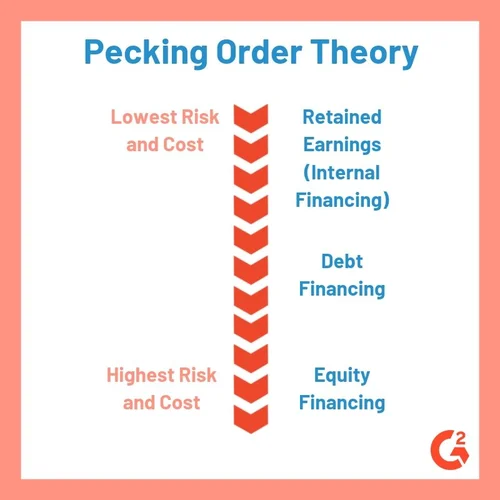
\includegraphics[width=\linewidth]{images/section3/peckingorder.png}
	\end{columns}
	
\end{frame}

\begin{frame}{Behavioral Implications of the Pecking Order}
	
	\textbf{Key Characteristics:}
	
	\begin{itemize}
		\item Firms do not target a specific debt-equity ratio.
		\item Capital structure evolves over time based on financing needs.
		\item More profitable firms tend to:
		\begin{itemize}
			\item Accumulate internal funds
			\item Avoid issuing equity
			\item Maintain low leverage
		\end{itemize}
		\item Firms value \textbf{financial slack}:
		\begin{itemize}
			\item Buffer to finance future investments
			\item Avoid negative signaling from external financing
		\end{itemize}
	\end{itemize}
	
\end{frame}

\begin{frame}{Pecking Order vs. Trade-Off Theory}
	
	\begin{table}[ht]
		\centering
		\resizebox{0.95\textwidth}{!}{
			\begin{tabular}{lcc}
				\toprule
				\textbf{Dimension} & \textbf{Trade-Off Theory} & \textbf{Pecking Order Theory} \\
				\midrule
				Key Driver & Tax benefits vs. distress cost & Information asymmetry \\
				Target D/E Ratio & Yes, optimal level exists & No target ratio \\
				Firm Behavior & Optimize WACC & Minimize info cost \\
				Leverage & Profitable firms use more debt & Profitable firms use less debt \\
				Focus & Long-run capital structure & Short-run financing tactics \\
				\bottomrule
			\end{tabular}
		}
	\end{table}
	
\end{frame}

\subsubsection{Dynamic Rebalancing Theory}
\begin{frame}{Dynamic Rebalancing Theory}
	
	\textbf{Do firms continuously adjust their capital structure toward an optimal level?}
	
	\begin{itemize}
		\item In theory (e.g., trade-off model), firms rebalance when leverage drifts from target.
		\item In reality, adjustments are \textbf{infrequent and partial}.
		\item Reasons for delayed rebalancing:
		\begin{itemize}
			\item Adjustment costs (transaction fees, signaling concerns)
			\item Managerial inattention or inertia
			\item Financial flexibility preferences
		\end{itemize}
		\item Empirical evidence:  
		\textcite{leary2005revolving} find most firms adjust slowly — often only when issuing external capital.
	\end{itemize}
	
	\vspace{0.3cm}
	\textbf{Implication:}  
	Observed leverage is often a result of past shocks and only gradually moves back toward target.
	
\end{frame}

\subsubsection{Market Timing Theory}
\begin{frame}{Market Timing Theory}
	
	\textbf{What if capital structure is just a by-product of timing past financing windows?}
	
	\begin{itemize}
		\item Firms issue equity when stock prices are high (perceived overvaluation).
		\item Firms issue debt when interest rates are low or stock price is undervalued.
		\item No target D/E ratio is needed — structure reflects historical timing.
	\end{itemize}
	
	\vspace{0.3cm}
	\textbf{Key Study:}  
	\textcite{baker2002market} show firms that issued equity during high valuations have persistently lower leverage over time.
	
	\vspace{0.3cm}
	\begin{alertblock}{Conclusion}
		Capital structure reflects \textbf{cumulative outcomes of past market conditions}, not just firm fundamentals.
	\end{alertblock}
	
\end{frame}

\subsubsection*{Alternative Capital Structure Theory}
\begin{frame}{Summary: Alternative Capital Structure Theories}
	
	\begin{table}[ht]
		\centering
		\resizebox{\textwidth}{!}{
			\begin{tabular}{lllll}
				\toprule
				\textbf{Theory} & \textbf{Key Driver} & \textbf{Mechanism} & \textbf{Prediction on Leverage} & \textbf{Notes} \\
				\midrule
				Agency Costs of Equity & Ownership–control sep & Equity dilution weakens managerial incentives & Higher debt improves effort alignment & \textcite{jensen1976theory} \\
				Free Cash Flow & Empire building risk & Debt limits managerial discretion & More debt when cash flow is high & \textcite{jensen1986agency} \\
				Signaling Theory & Private info asymmetry & High-quality firms use more debt & High debt = high quality signal & \textcite{ross1977signaling} \\
				Pecking Order Theory & Info asymmetry + cost & Internal > debt > equity & Profitable firms use less debt & \textcite{myers1984corporate} \\
				Dynamic Rebalancing & Adjustment costs & Partial, slow return to target & D/E drifts over time & \textcite{leary2005revolving} \\
				Market Timing Theory & Valuation windows & Issue equity when overvalued & Structure reflects timing history & \textcite{baker2002market} \\
				\bottomrule
			\end{tabular}
		}
	\end{table}
	
	\vspace{0.2cm}
	\textbf{Conclusion:} These theories complement the traditional trade-off framework by incorporating behavior, information, and dynamics.
	
\end{frame}


\subsection{How Firms Establish Capital Structure in Practice}
\begin{frame}{Capital Structures Vary Widely Across Countries}
	
	\begin{figure}
		\centering
		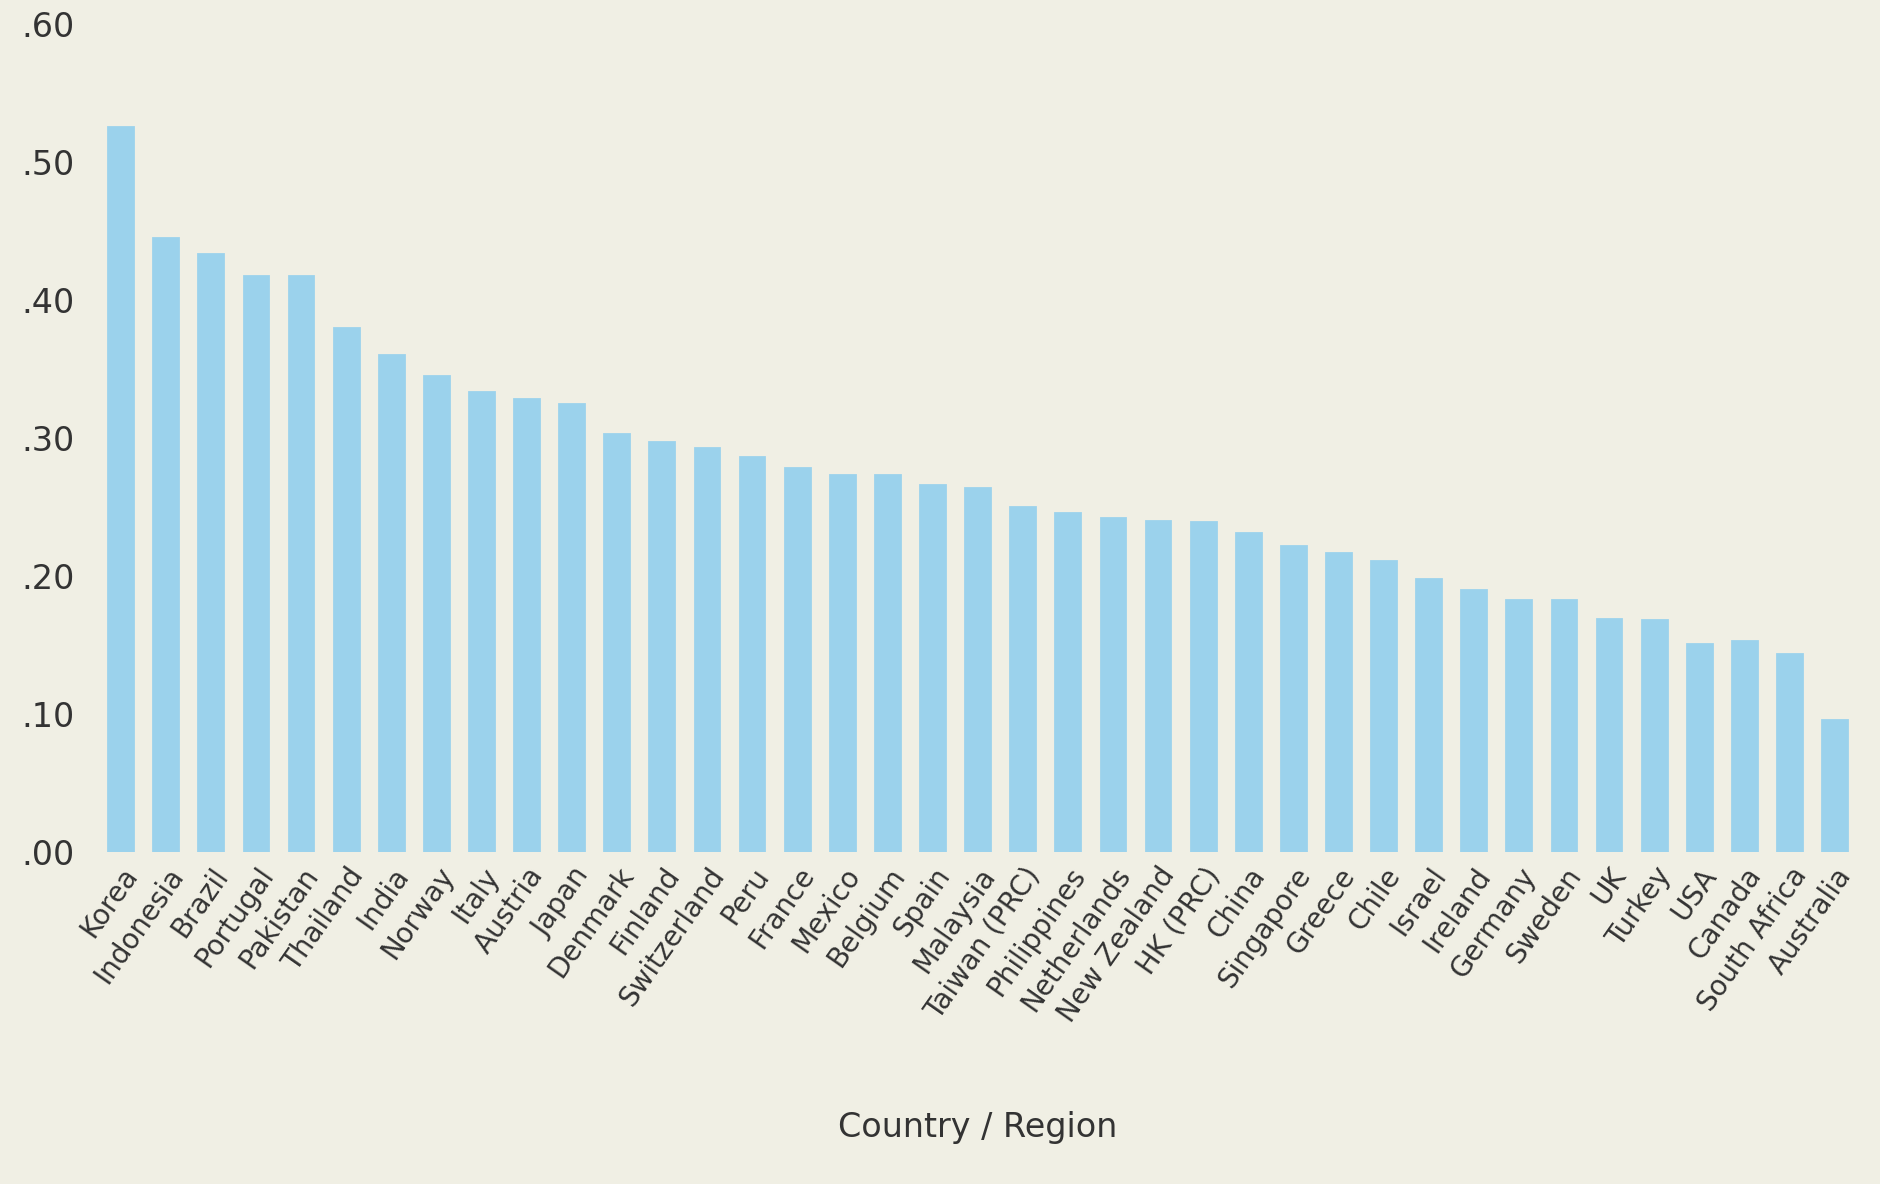
\includegraphics[width=0.85\textwidth]{images/section3/internationaldbratio.png}
	\end{figure}
	
	\tiny{Source: \textcite{fan2012international}. Shows median debt-to-assets ratios across countries.}
	
	\textbf{Observation:} Even in the absence of global theory consensus, capital structure is influenced by tax laws, legal protections, and institutional quality.
\end{frame}
\begin{frame}{Most Firms Maintain a Target Capital Structure}
	
	\begin{figure}
		\centering
		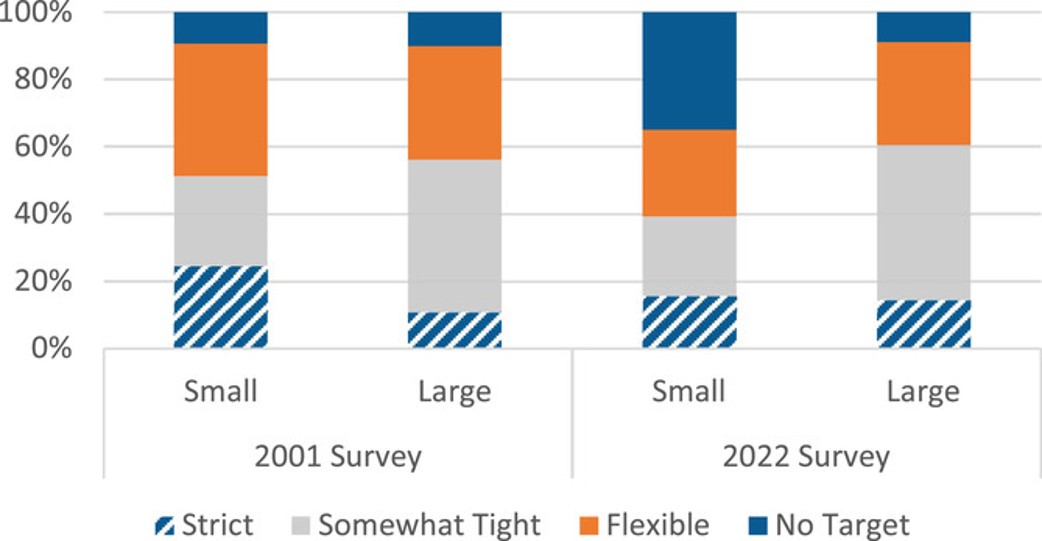
\includegraphics[width=0.85\textwidth]{images/section3/targetdebt.jpg}
	\end{figure}
	
	\tiny{Source: \textcite{graham2022presidential}. Survey evidence: Firms differ in how strictly they follow D/E targets.}
	
	\vspace{2mm}
	\textbf{Key Insight:} Most firms (especially large ones) maintain a target debt ratio — but many adopt flexible or somewhat loose adherence.
\end{frame}
\begin{frame}{Firm-Level Capital Structures Are Not Static}
	
	\begin{columns}
		% Left: Image
		\begin{column}{0.4\textwidth}
			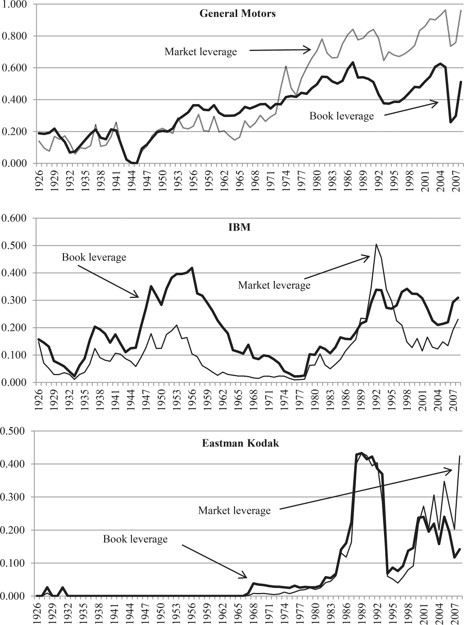
\includegraphics[width=\linewidth]{images/section3/csvariation.jpg}\\
			\tiny{Source: \textcite{deangelo2015stability}}
		\end{column}
		
		% Right: Text
		\begin{column}{0.6\textwidth}
			\textbf{Key Insight:} \\
			Capital structure targets are often long-term — in the short run, observed leverage can deviate significantly.
			
			\vspace{0.4cm}
			\textbf{Why does leverage drift?}
			\begin{itemize}
				\item Changes in market equity value (denominator)
				\item Internal equity financing via retained earnings
				\item No immediate need to rebalance
			\end{itemize}
			
			\vspace{0.3cm}
			\textbf{Implication:} Leverage ratios are dynamic, even for firms with long-run targets.
		\end{column}
	\end{columns}
	
\end{frame}

\begin{frame}{Capital Structures Differ by Industry}
	
	\begin{figure}
		\centering
		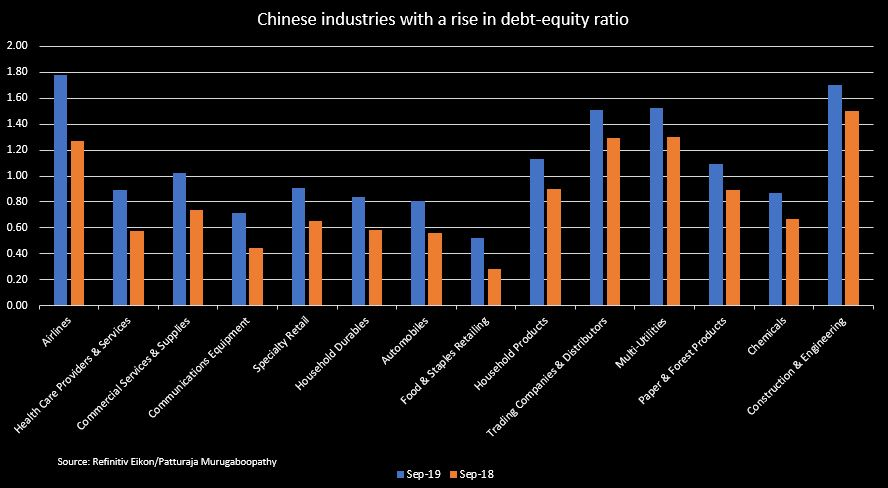
\includegraphics[width=0.9\textwidth]{images/section3/cnderatio.jpg}
	\end{figure}
	
	\tiny{Source: Refinitiv / Reuters. Leverage varies based on operating risk and asset type.}
	
	\vspace{2mm}
	\textbf{Example:} Airlines and utilities exhibit high leverage; tech and services often rely more on equity.
\end{frame}
\begin{frame}{What Determines a Firm’s Target D/E Ratio?}
	
	\begin{itemize}
		\item \textbf{Taxes:}
		\begin{itemize}
			\item Interest tax shield encourages more debt for profitable firms.
		\end{itemize}
		
		\item \textbf{Asset Tangibility:}
		\begin{itemize}
			\item Tangible assets provide collateral → lower distress costs → higher debt capacity.
			\item Firms with intangible assets (e.g., R\&D) favor equity.
		\end{itemize}
		
		\item \textbf{Earnings Volatility:}
		\begin{itemize}
			\item More volatile EBIT increases risk of distress → encourages equity financing.
		\end{itemize}
	\end{itemize}
	
	\vspace{2mm}
	\textbf{Additional factors:} growth opportunities, managerial preferences, macro conditions.
	
\end{frame}
\begin{frame}{Empirical Realities of Capital Structure: Key Takeaways}
	
	\begin{itemize}
		\item \textbf{Capital structure is context-specific} — shaped by:
		\begin{itemize}
			\item Institutional environment (e.g., legal systems, taxation)
			\item Industry characteristics (e.g., asset tangibility, volatility)
			\item Firm attributes (e.g., size, profitability, lifecycle stage)
		\end{itemize}
		
		\item \textbf{Target leverage ratios exist}, but are often flexible bands rather than precise points.
		
		\item \textbf{Observed capital structure fluctuates} due to:
		\begin{itemize}
			\item Market valuation changes
			\item Internal financing and retained earnings
			\item Timing or adjustment costs
		\end{itemize}
		
		\item \textbf{Theory provides a framework}, but real-world capital structure reflects both rational design and practical constraints.
	\end{itemize}
	
\end{frame}

\subsection*{Summary}
\begin{frame}{Summary: Capital Structure and Its Limits}
	\footnotesize
	\textbf{1. Why Not 100\% Debt?} \\
	\begin{itemize}
		\item Debt provides tax shields, but...
		\item \textcolor{red}{Bankruptcy costs} (direct + indirect) reduce firm value
		\item \textcolor{red}{Agency conflicts} (e.g., risk-shifting, underinvestment)
	\end{itemize}
	
	\textbf{2. Main Theories Beyond MM} \\
	\begin{itemize}
		\item \textbf{Trade-Off Theory:} Balance tax benefits and distress costs
		\item \textbf{Agency Theory:} Debt disciplines managers; equity dilutes incentives
		\item \textbf{Signaling Theory:} High leverage = signal of firm quality
		\item \textbf{Pecking Order:} Internal $>$ Debt $>$ Equity (due to asymmetric info)
		\item \textbf{Market Timing \& Rebalancing:} Structure reflects past opportunities
	\end{itemize}
	
	\textbf{3. Real-World Implications} \\
	\begin{itemize}
		\item Most firms maintain flexible target ranges for D/E
		\item Leverage varies across \textbf{countries, industries, firm types}
		\item Capital structure reflects both \textit{rational design} and \textit{practical constraints}
	\end{itemize}
	
\end{frame}

\begin{frame}{Discussion: Which Theory Best Fits China?}
	
	\textbf{Question:}  
	Which capital structure theory best explains the financing behavior of firms in China?
	
	\begin{itemize}
		\item \textbf{Trade-Off Theory}
		\begin{itemize}
			\item Does the tax shield dominate firm decisions?
			\item How important are bankruptcy costs in SOEs vs. private firms?
		\end{itemize}
		
		\item \textbf{Pecking Order Theory}
		\begin{itemize}
			\item Do firms avoid equity due to asymmetric information?
			\item What is the role of internal funds and retained earnings?
		\end{itemize}
		
		\item \textbf{Agency / Free Cash Flow}
		\begin{itemize}
			\item How does concentrated ownership affect managerial behavior?
			\item Are high cash firms more likely to over-invest?
		\end{itemize}
		
		\item \textbf{Market Timing}
		\begin{itemize}
			\item Do Chinese firms issue equity in “hot” markets?
			\item Are IPO waves driven by valuation windows?
		\end{itemize}
	\end{itemize}
	
	\textbf{Follow-up:}  
	Can one theory explain all firms? Or do different types (SOEs, tech, exporters) follow different models?
	
\end{frame}
